% CREATED BY DAVID FRISK, 2015
\chapter{Theory}
\textbf{How Conflicts Arise in a GIT-based Branching and Merging Scenario.} Many software projects follow a branching model when using Git, such as the one explained by Giessen [2]. In these models, users create feature branches that provide an environment where new features can be implemented and tested without affecting the end-user version of the software [3]. There are various ways to use branches. A branch can be created for each new feature, for each new release, and for each product [1]. When a new feature has been implemented in a new branch, the branch needs to be merged into another branch, such as the main branch. Merging is the process of joining two branches together, both in case of two local branches or a local and a remote branch [4]. At GitHub, this is usually done using a pull request. A pull request is made to let the collaborators in the repository know that the commits in a branch are ready to be merged. The collaborators can review the new code and input their feedback until it is finally approved for merging into the end-user branch [5]. Merging can also be performed without using pull requests. When branches are to be merged, conflicts might arise. Conflicts are the problems that prevent git from automatically merging two branches together.

\paragraph*{}
\textbf{Problems of Resolving Merge Conflicts.} Resolving merge conflicts, such as those arising from changes to different variants of features, is difficult. Merging might require refactoring the class hierarchy, introducing design patterns, or adding parameters to the feature. If it would be possible to develop an autonomous tool that can provide automated conflict resolution in this case, it would be of great value, since resolving such conflicts is a recurring problem that is solved manually today. The problem is that the development of such a tool requires more understanding of how the merge-conflict resolution is performed. Hence, in the scenario above, we’re interested in studying merge-conflict resolutions.

\paragraph*{}
\textbf{Problems of an Empirical Study of Conflict Resolutions.} However, even that is difficult. It is unclear whether and how we could study such resolutions as they are performed by developers in real-world software. For having representative results, one would also need to study the resolutions in large codebases, such as from GitHub/BitBucket. This requires some automated analysis. It is not trivial how this automated analysis could be designed. It is also unclear how many projects can be studied; it’s even not clear which projects are well-suited for such a study.

\paragraph*{}
\textbf{Problem Reports and Empirical Studies.} Cloning happens during all stages of a software-development process, and it is the responsibility of the developers themselves to make sure that changes between copies of the clones are propagated correctly [1]. Because of this, there are risks that conflicts arise during all stages of the development process.

\paragraph*{}
With the use of a version control system, cloning can be managed in a more smooth way by using branching and merging capabilities [6]. GitHub uses the version control system Git, which maintains a development history for each project. In this history lies the information about when merges have occurred. When cloning features, multiple versions of the same feature exists and their consistency needs to be managed [6].

\paragraph*{}
\textbf{Textual Merging.} The most commonly used merging technique is textual merging [7]. Textual merging is based on the history and on textual differences. It does not make use of any knowledge of the syntax or semantic. One must also distinguish between two-way merging and three-way merging. In two-way merging, only the two conflicting clones are analyzed to resolve the conflict. In three-way merging, also the common ancestor is used, which is more powerful [8].

\paragraph*{}
\textbf{Semistructured Merging.}Semistructured Merging. Furthermore, there exist merge tools that uses another approach than textual merging, such as syntactic- and semantic merging, which have language specific knowledge [9] and does not only compare lines of text. A combination of both textual merging, syntactic and semantic merging is called semistructured merging [7]. Other studies have proved that the use of semistructured merge decreases the number of conflicts significantly. The study “Assessing Semistructured Merge in Version Control Systems: A Replicated Experiment”, proves that semistructured merge can reduce the number of conflicts by 55\% [10]. These works are important to us. But instead of proposing a new conflict-resolution technique, we are interested in how developers resolve conflicts arising from different variants of features or projects.

\paragraph*{}
\textbf{Conflict Patterns.} During merging, several types of conflict patterns might occur. In her study, Accioly [11] identifies numerous conflict patterns. This list will be used throughout our study both to learn about which conflict patterns exist, and later using them when developing the analyzing tool. While Accioly focuses conflict patterns, we strive to identify conflict-resolution patterns.

\paragraph*{}
\textbf{Mining.} To automatically analyze projects on GitHub, a high number of requests to GitHub has to be performed. When querying requests to GitHub, GitHub has a limit of 5000 requests per hour [12]. 


%In the following sections, examples of a figure, an equation, a table, a chemical structure, a list, a listing and a to-do note are shown.

\section{Figure}
\begin{figure}[H]
\centering
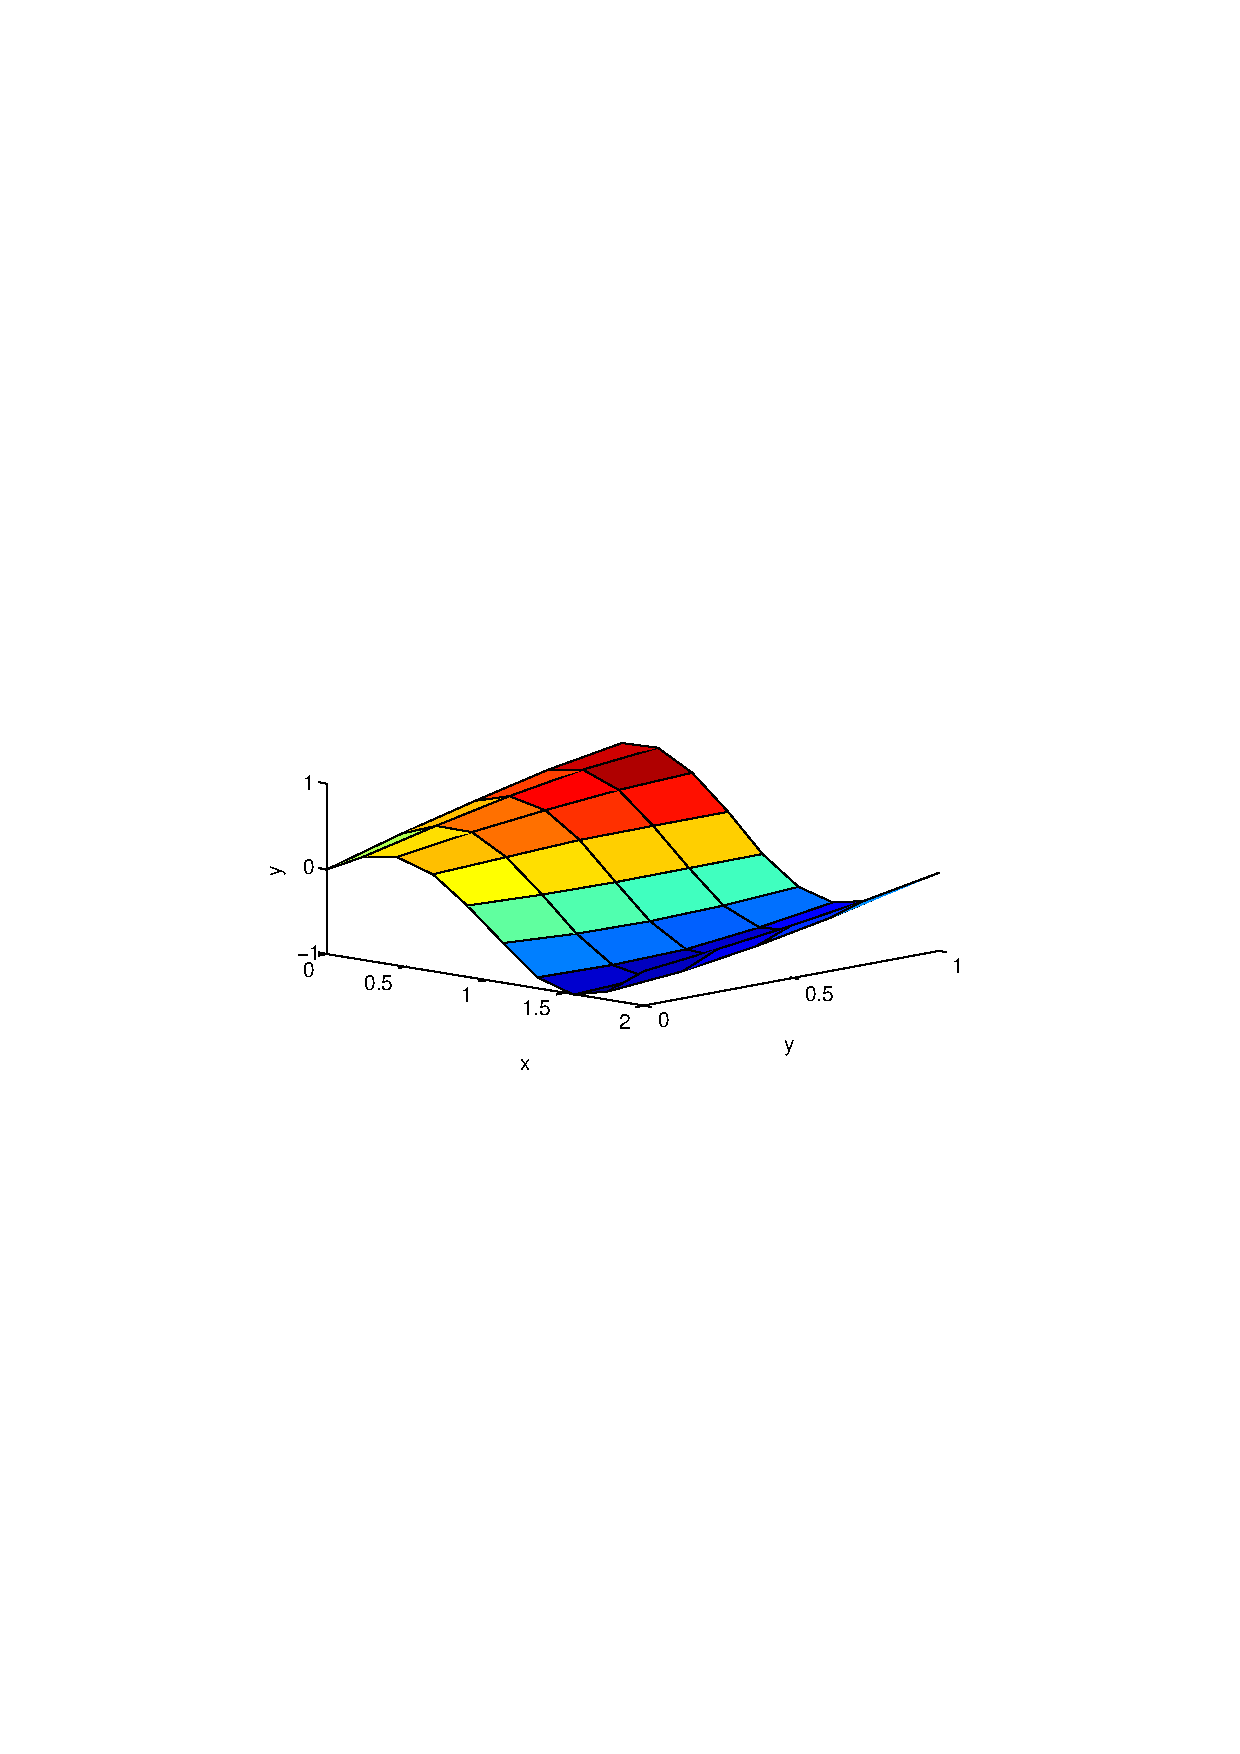
\includegraphics[width=0.45\linewidth, trim=3cm 11cm 3cm 11cm]{figure/X.pdf}
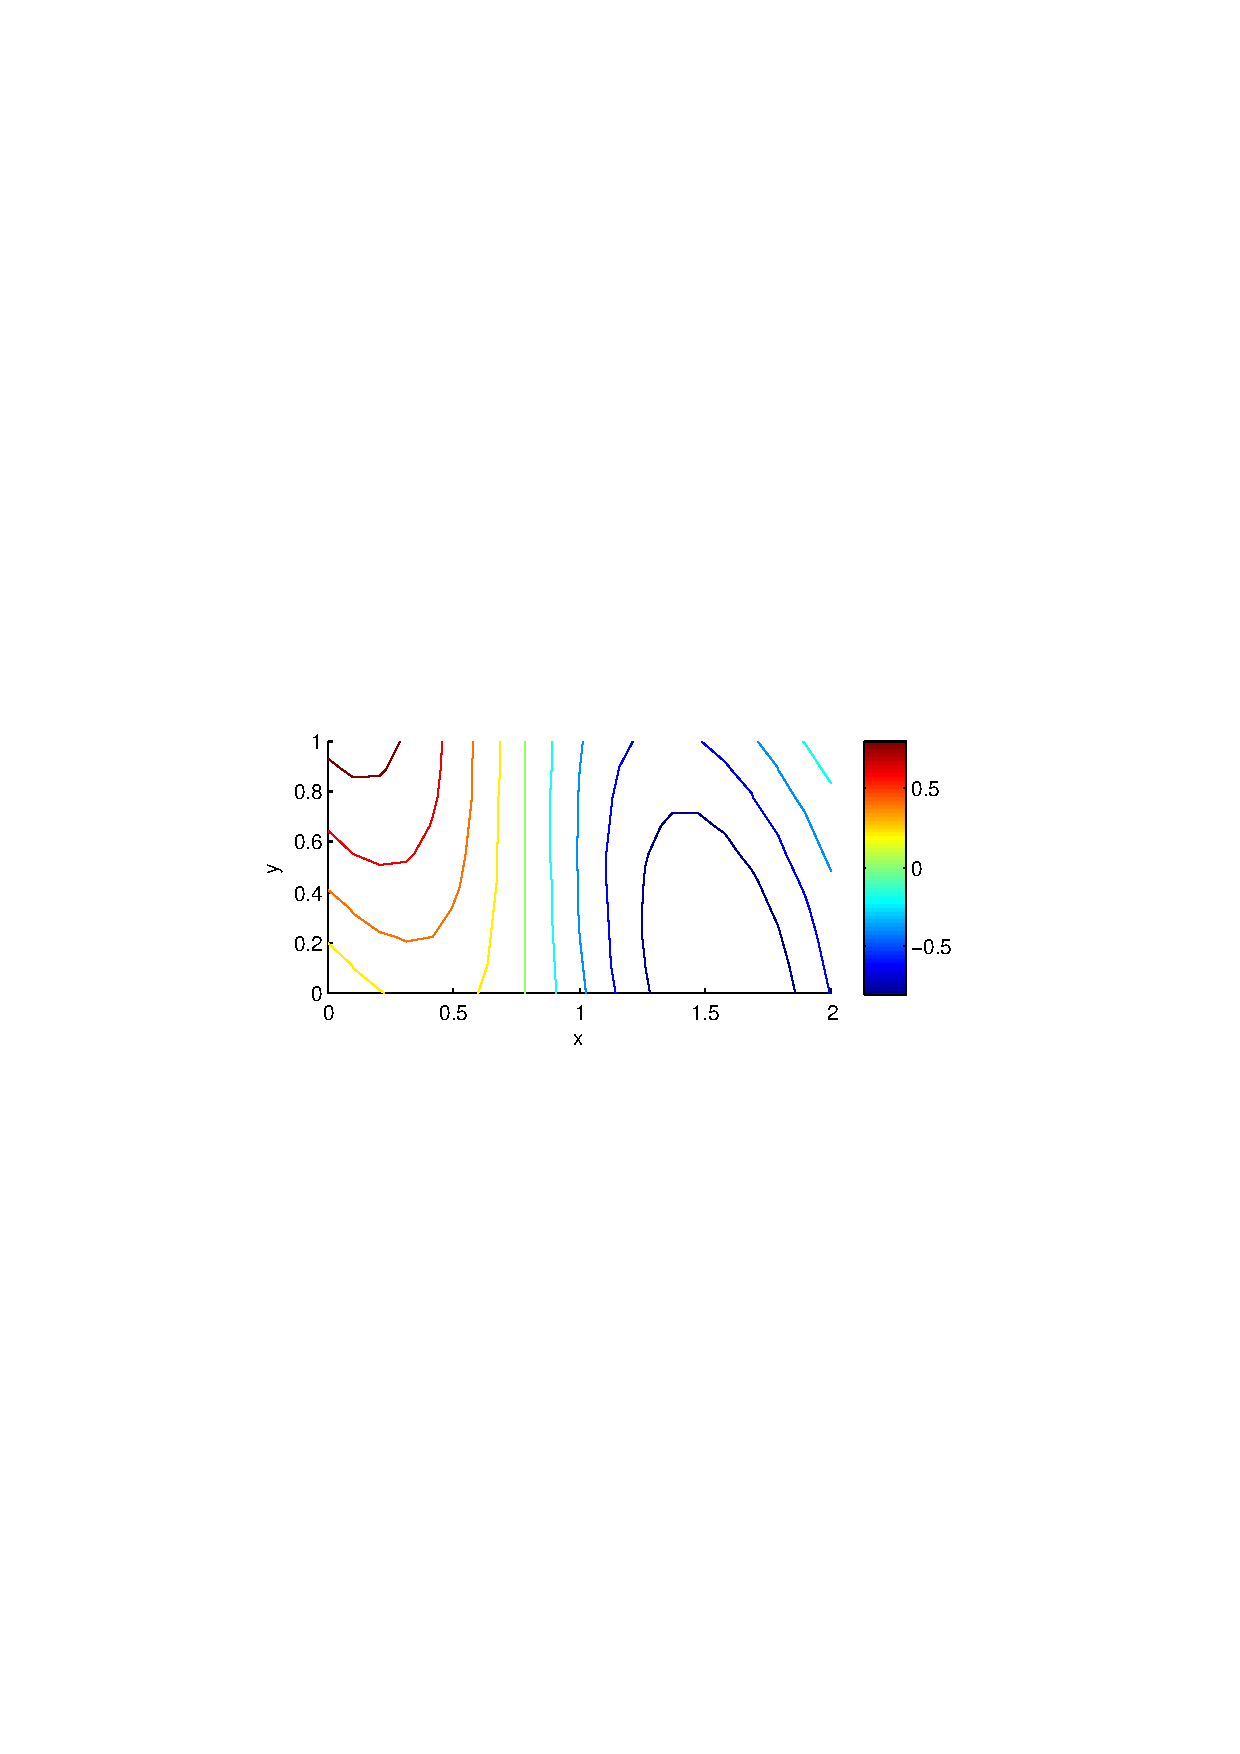
\includegraphics[width=0.45\linewidth, trim=3cm 11cm 3cm 11cm]{figure/Y.pdf}
\caption{Surface and contour plots showing $z(x,y)=\sin(x+y)\cos(2x)$.}
\end{figure}

\section{Equation}
\begin{equation}
f(t)=\left\{ \begin{array}{ll}
1,~~~~ & t< 1 \\
t^2 & t\geq 1
\end{array}\right.
\end{equation}

\section{Table}
\begin{table}[H]
\centering
\caption{Values of $f(t)$ for $t=0,1,\dots 5$.}
\begin{tabular}{l|llllll} \hline\hline
$t$ & 0 & 1 & 2 & 3 & 4 & 5 \\ \hline
$f(t)$ & 1 & 1 & 4 & 9 & 16 & 25 \\ \hline\hline
\end{tabular}
\end{table}

\section{Chemical structure}
\begin{center}
\chemfig{X*5(-E-T-A-L-)}
\end{center}

\section{List}
\begin{enumerate}
  \item The first item
  \begin{enumerate}
    \item Nested item 1
    \item Nested item 2
  \end{enumerate}
  \item The second item
  \item The third item 
  \item \dots
\end{enumerate}

\section{Source code listing}
%\lstset{language=Matlab}
\begin{lstlisting}[frame=single]
% Generate x- and y-nodes
x=linspace(0,1); y=linspace(0,1);

% Calculate z=f(x,y)
for i=1:length(x)
 for j=1:length(y)
  z(i,j)=x(i)+2*y(j);
 end
end
\end{lstlisting}

\section{To-do note}
The \texttt{todo} package enables to-do notes to be added in the page margin. This can be a very convenient way of making notes in the document during the process of writing. All notes can be hidden by using the option \emph{disable} when loading the package in the settings. \todo{Example of a to-do note.}

